\section{Actores}

A continuación se describen los actores que se involucran, de una manera u otra,
con el sistema.

\begin{description}

\item[Cliente] \hfill \\
Solicita una tarjeta y realiza compras con ella.

\item[Comercio] \hfill \\
Realiza ventas de bienes y/o servicios al cliente, quien paga por ellos
utilizando la tarjeta.

\item[Administrador] \hfill \\
Configura y administra el sistema informático desarrollado manteniendo datos de
referencia como ser los comercios y clientes registrados.

\item[Mensualmente] \hfill \\
Actor temporal mensual involucrado en los procesos de generación de resúmenes de
cuenta por clientes y resúmenes de saldo por comercio.

\item[Diariamente] \hfill \\
Actor temporal diario involucrado en los procesos de verificación y renovación
de tarjetas vencidas.

\end{description}

\section{Diagrama de casos de uso} \label{sec:diagrama_casos_uso}

En la figura~\ref{fig:modcasosuso:diagramacasos} se exponen los actores
involucrados en la operación del sistema y su interacción con el mismo a través
de los casos de uso identificados. En secciones subsiguientes se detallará cada
uno de estos últimos.

\begin{figure}[htb]
\begin{center}
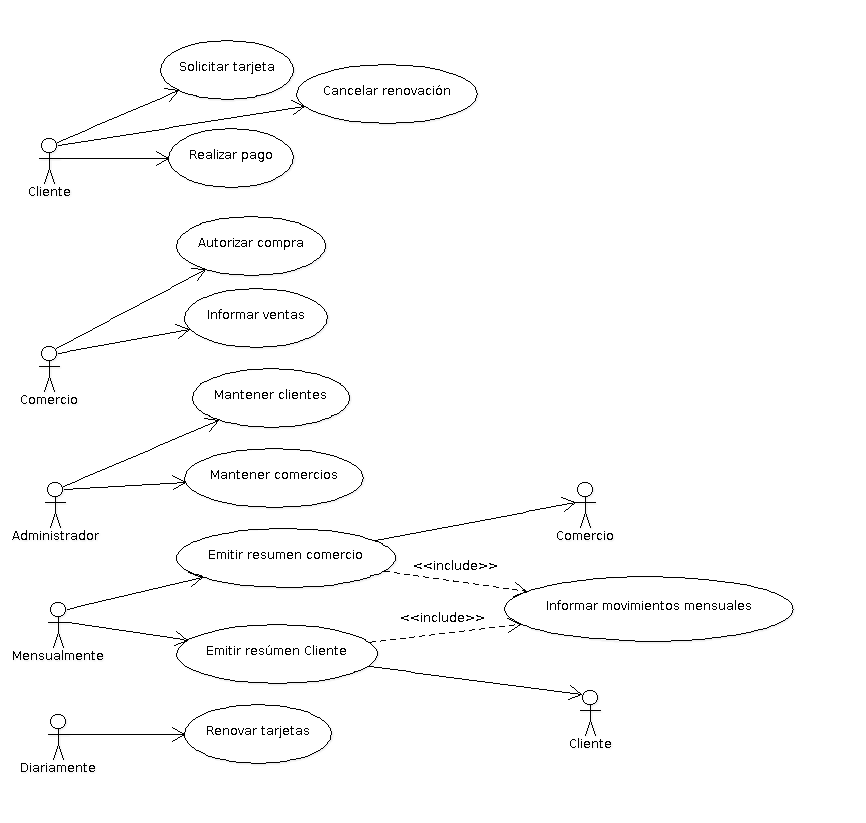
\includegraphics[width=0.9\textwidth]{images/mod_casosuso_diagrama.png}
\end{center}
\caption{Diagrama de casos de uso}
\label{fig:modcasosuso:diagramacasos}
\end{figure}

\FloatBarrier

\section{Detalle de casos de uso}

En esta sección se detallan cada uno de los casos de uso presentados en el
diagrama de casos de uso de la sección~\ref{sec:diagrama_casos_uso}.

\subsection{Solicitar tarjeta}
\begin{tabularx}{\textwidth}{| r | X |}
\hline
\multicolumn{2}{|X|}{
\textbf{Use Case}: Solicitar tarjeta} \\

\hline
\multicolumn{2}{|c|}{\cellcolor[gray]{0.6}} \\

\hline
\multicolumn{2}{|X|}{
\textbf{Descripción}: Registración de los datos de un cliente y emisión de una
tarjeta a su nombre.} \\

\hline
\multicolumn{2}{|X|}{
\textbf{Actores participantes}: Cliente} \\

\hline
\multicolumn{2}{|c|}{\cellcolor[gray]{0.6} } \\

\hline
\multicolumn{2}{|X|}{
\textbf{Flujos}} \\

\hline
\multicolumn{2}{|X|}{
\textbf{Flujo principal}} \\

\hline
1 & El cliente solicita una nueva tarjeta. \\
\hline
2 & El sistema solicita los datos del cliente. \\
\hline
3 & Se ingresan los datos del cliente (nombre, apellido, dni, límite de compra,
domicilio, teléfono). \\
\hline
4 & El sistema valida que el dni del cliente no haya sido registrado aún (E1.1
si ya ha sido registrado). \\
\hline
5 & El sistema pide confirmación de que el cliente ha presentado una fotocopia
de su dni (E2.1 si no se da confirmación). \\
\hline
6 & El sistema pide confirmación de que el cliente ha presentado la
documentación asociada a la garantía, y que esta es satisfactoria (E2.1 si no se
da confirmación). \\
\hline
7 & El sistema almacena los datos del cliente y genera un número de tarjeta. \\
\hline
8 & Fin del caso de uso. \\

\hline
\multicolumn{2}{|X|}{
\textbf{Flujos de excepción}} \\

\hline
E1.1 & El sistema emite un mensaje de error informando que el cliente ya posee
una tarjeta. \\
\hline
E1.2 & El caso de uso continua en 8 \\

\hline
E2.1 & El sistema emite un mensaje de error informando que el cliente no
presentó documentación obligatoria para continuar con la solicitud. \\
\hline
E1.2 & El caso de uso continua en 8 \\

\hline
\end{tabularx}



\subsection{Cancelar renovación}
\begin{tabularx}{\textwidth}{| r | X |}
\hline
\multicolumn{2}{|X|}{
\textbf{Use Case}: Cancelar renovación} \\

\hline
\multicolumn{2}{|c|}{\cellcolor[gray]{0.6}} \\

\hline
\multicolumn{2}{|X|}{
\textbf{Descripción}: Cancela el proceso de renovación automática de la tarjeta,
de manera que la tarjeta sigue vigente hasta que expire. A partir de su
expiración, la tarjeta se mantiene como inactiva y no puede ser utilizada.} \\

\hline
\multicolumn{2}{|X|}{
\textbf{Actores participantes}: Cliente} \\

\hline
\multicolumn{2}{|c|}{\cellcolor[gray]{0.6} } \\

\hline
\multicolumn{2}{|X|}{
\textbf{Flujos}} \\

\hline
\multicolumn{2}{|X|}{
\textbf{Flujo principal}} \\

\hline
1 & El cliente solicita la cancelación de la renovación automática de su
tarjeta. \\
\hline
2 & El sistema solicita el número de tarjeta del cliente. \\
\hline
3 & El sistema valida que el número de tarjeta del cliente exista (E1.1 si no
existe). \\
\hline
4 & El sistema valida que la tarjeta del cliente esté activa y su renovación no
haya sido cancelada (E2.1 si está inactiva o su renovación ya ha sido
cancelada). \\
\hline
5 & El sistema marca la tarjeta como "no renovar". Se mantiene activa, pero en
su fecha de expiración la tarjeta no se renovará automáticamente. \\
\hline
6 & Fin del caso de uso. \\

\hline
\multicolumn{2}{|X|}{
\textbf{Flujos de excepción}} \\

\hline
E1.1 & El sistema emite un mensaje de error informando que no existe una tarjeta
con el número de tarjeta ingresado \\
\hline
E1.2 & El caso de uso continua en 6 \\

\hline
E2.1 & El sistema emite un mensaje de error informando que la tarjeta está
inactiva o que su renovación ya ha sido cancelada. \\
\hline
E2.2 & El caso de uso continua en 6 \\

\hline
\end{tabularx}



\subsection{Realizar pago}
\begin{tabularx}{\textwidth}{| r | X |}
\hline
\multicolumn{2}{|X|}{
\textbf{Use Case}: Realizar pago} \\

\hline
\multicolumn{2}{|c|}{\cellcolor[gray]{0.6}} \\

\hline
\multicolumn{2}{|X|}{
\textbf{Descripción}: Registración de un pago a nombre de un cliente en
concepto de los consumos realizados durante el mes anterior.} \\

\hline
\multicolumn{2}{|X|}{
\textbf{Actores participantes}: Cliente} \\

\hline
\multicolumn{2}{|c|}{\cellcolor[gray]{0.6} } \\

\hline
\multicolumn{2}{|X|}{
\textbf{Flujos}} \\

\hline
\multicolumn{2}{|X|}{
\textbf{Flujo principal}} \\

\hline
1 & El cliente se presenta en las oficinas de pagos para pagar el monto
adeudado. \\
\hline
2 & El sistema solicita el DNI del cliente. (E1 si el cliente no existe). \\
\hline
3 & El sistema informa los datos del cliente para su validación, y solicita
confirmación de que estos son correctos (E2 si los datos no son correctos). \\
\hline
4 & El sistema informa el monto adeudado por el cliente. (S1 si el monto
adeudado es cero, S2 si la fecha del día no es del uno al diez de cada mes). \\
\hline
5 & El sistema solicita el importe abonado por el cliente y actualiza el saldo
de su cuenta corriente.\\
\hline
6 & Fin del caso de uso. \\

\hline
\multicolumn{2}{|X|}{
\textbf{Flujos alternativos}} \\

\hline
S1.1 & El sistema emite un mensaje informando que el cliente no posee saldo
adeudado. \\
\hline
S1.2 & El caso de uso continua en 6. \\

\hline
S2.1 & El sistema emite un mensaje informando que no se pueden registrar pagos
fuera de término, e indicando el próximo periodo en el que se podrán registrar
pagos (en las fechas uno al diez de cada mes). \\
\hline
S2.2 & El caso de uso continua en 6. \\


\hline
\multicolumn{2}{|X|}{
\textbf{Flujos de excepción}} \\

\hline
E1.1 & El sistema emite un mensaje de error informando que el cliente no
existe. \\
\hline
E1.2 & El caso de uso continua en 6. \\

\hline
E2.1 & El sistema emite un mensaje de error informando que no se registrará
ningún pago. \\
\hline
E2.2 & El caso de uso continua en 2. \\

\hline
\end{tabularx}



\subsection{Autorizar compra}
\begin{tabularx}{\textwidth}{| r | X |}
\hline
\multicolumn{2}{|X|}{
\textbf{Use Case}: Autorizar compra} \\

\hline
\multicolumn{2}{|c|}{\cellcolor[gray]{0.6}} \\

\hline
\multicolumn{2}{|X|}{
\textbf{Descripción}: Validación de las condiciones de uso de una tarjeta para
realizar un pago en un comercio adherido.} \\

\hline
\multicolumn{2}{|X|}{
\textbf{Actores participantes}: Comercio} \\

\hline
\multicolumn{2}{|c|}{\cellcolor[gray]{0.6} } \\

\hline
\multicolumn{2}{|X|}{
\textbf{Flujos}} \\

\hline
\multicolumn{2}{|X|}{
\textbf{Flujo principal}} \\

\hline
1 & El comercio requiere al sistema que este valide una tarjeta informando el
número de esta, el DNI del cliente y el importe de la venta que el cliente
quiere abonar utilizando la misma. \\
\hline
2 & El sistema realiza las siguientes validaciones (S1 si alguna de las
validaciones fallase). 
\begin{enumerate}
\item El número de tarjeta debe estar asociado a una tarjeta.
\item La tarjeta debe estar activa.
\item El DNI del cliente asociado a la tarjeta debe coincidir con el DNI
informado.
\item El saldo de la cuenta asociada a la tarjeta más el importe informado de
la venta no debe superar el límite de saldo asociado a la cuenta.
\end{enumerate} \\
\hline
3 & El sistema informa al comercio que la compra está autorizada. \\
\hline
4 & Fin del caso de uso. \\

\hline
\multicolumn{2}{|X|}{
\textbf{Flujos alternativos}} \\

\hline
S1.1 & El sistema informa al comercio que la compra no está autorizada,
adjuntando en el mensaje el motivo por el cual no se autoriza la misma. \\
\hline
S1.2 & El caso de uso continua en 4. \\

\hline
\end{tabularx}



\subsection{Informar ventas}
\begin{tabularx}{\textwidth}{| r | X |}
\hline
\multicolumn{2}{|X|}{
\textbf{Use Case}: Informar ventas} \\

\hline
\multicolumn{2}{|c|}{\cellcolor[gray]{0.6}} \\

\hline
\multicolumn{2}{|X|}{
\textbf{Descripción}: Registración de las ventas sumarizadas por día en un
comercio particular.} \\

\hline
\multicolumn{2}{|X|}{
\textbf{Actores participantes}: Comercio} \\

\hline
\multicolumn{2}{|c|}{\cellcolor[gray]{0.6} } \\

\hline
\multicolumn{2}{|X|}{
\textbf{Flujos}} \\

\hline
\multicolumn{2}{|X|}{
\textbf{Flujo principal}} \\

\hline
1 & El comercio informa las ventas realizadas a los distintos clientes en un
día particular, proporcionando la fecha para la cual se están informando las
ventas, el código del comercio que las está informando y un listado que indica
el número de tarjeta y el importe sumarizado de todas las ventas en la fecha
informada para dicha tarjeta.\\
\hline
2 & El realiza las siguientes validaciones (E1 si alguna de ellas fallase). 
\begin{enumerate}
\item Debe existir un comercio con el código de comercio informado.
\item La fecha proporcionada debe corresponder al mes actual.
\item Los números de tarjeta proporcionados deben estar todos asociados cada
uno a una tarjeta activa.
\end{enumerate}
\\
\hline
3 & El sistema registra las transacciones informadas. \\
\hline
4 & Fin del caso de uso. \\

\hline
\multicolumn{2}{|X|}{
\textbf{Flujos de excepción}} \\

\hline
E1.1 & El sistema emite un mensaje de error informando que los datos informados
son incorrectos, adjuntando un mensaje que indica la validación que falló. \\
\hline
E1.2 & El caso de uso continua en 4. \\

\hline
\end{tabularx}



\subsection{Mantener clientes}
\begin{tabularx}{\textwidth}{| r | X |}
\hline
\multicolumn{2}{|X|}{
\textbf{Use Case}: Mantener clientes} \\

\hline
\multicolumn{2}{|c|}{\cellcolor[gray]{0.6}} \\

\hline
\multicolumn{2}{|X|}{
\textbf{Descripción}: Mantenimiento de la información relacionada a los
clientes.} \\

\hline
\multicolumn{2}{|X|}{
\textbf{Actores participantes}: Administrador} \\

\hline
\multicolumn{2}{|c|}{\cellcolor[gray]{0.6} } \\

\hline
\multicolumn{2}{|X|}{
\textbf{Flujos}} \\

\hline
\multicolumn{2}{|X|}{
\textbf{Flujo principal}} \\

\hline
1 & El sistema solicita el DNI, nombre, apellido o teléfono del cliente. \\
\hline
2 & El administrador proporciona cualquier combinación de los campos
solicitados (por ejemplo, proporcionando nombre y apellido, o sólo nombre, o
teléfono y DNI, etc.). \\
\hline
3 & El sistema valida que se haya proporcionado información en al menos uno de
los campos (E1 si no se proporcionó ninguna información). \\
\hline
4 & El sistema realiza una búsqueda de todos los clientes registrados cuya
información coincida, aunque sea parcialmente, con los datos proporcionados. \\
\hline
5 & El sistema muestra un listado con todos los clientes cuya información
coincide, al menos parcialmente, con la información proporcionada. Dicho
listado debe incluir DNI, nombre, apellido y teléfono del cliente. Por cada
cliente, el sistema proporciona la opción de modificar dicha información. (S1
si el administrador elige la opción de modificar el cliente). \\
\hline
6 & Fin del caso de uso. \\

\hline
\multicolumn{2}{|X|}{
\textbf{Flujos alternativos}} \\

\hline
S1.1 & El sistema solicita el nombre, apellido, DNI, límite de compra,
domicilio, teléfono y número de tarjeta, completando por defecto cada dato con
el valor almacenado actualmente en el sistema para el cliente. \\
\hline
S2.1 & El sistema almacena los nuevos valores de cada campo para el cliente. \\
\hline
S1.2 & El caso de uso continua en 6. \\

\hline
\multicolumn{2}{|X|}{
\textbf{Flujos de excepción}} \\

\hline
1.1 & El sistema muestra un mensaje de error indicando que debe completarse al
menos uno de los criterios de búsqueda. \\
\hline
1.2 & El caso de uso continua en 6. \\


\hline
\end{tabularx}



\subsection{Mantener comercios}
\begin{tabularx}{\textwidth}{| r | X |}
\hline
\multicolumn{2}{|X|}{
\textbf{Use Case}: Mantener comercios} \\

\hline
\multicolumn{2}{|c|}{\cellcolor[gray]{0.6}} \\

\hline
\multicolumn{2}{|X|}{
\textbf{Descripción}: Mantenimiento de la información relacionada a los
comercios.} \\

\hline
\multicolumn{2}{|X|}{
\textbf{Actores participantes}: Administrador} \\

\hline
\multicolumn{2}{|c|}{\cellcolor[gray]{0.6} } \\

\hline
\multicolumn{2}{|X|}{
\textbf{Flujos}} \\

\hline
\multicolumn{2}{|X|}{
\textbf{Flujo principal}} \\

\hline
1 & El sistema despliega las opciones de Alta, Baja o Consulta. \\
\hline
2 & El administrador elige una opción. (S1 para alta, S2 para baja, S3 para
consulta). \\
\hline
3 & Fin del caso de uso. \\

\hline
\multicolumn{2}{|X|}{
\textbf{Flujos alternativos}} \\

\hline
S1.1 & El sistema solicita los datos del comercio (nombre y código). \\
\hline
S1.2 & El administrador ingresa los datos solicitados. \\
\hline
S1.3 & El sistema valida que el código no esté asociado a otro comercio
preexistente (E1 si el código ya está asociado a otro comercio). \\
\hline
S1.4 & El sistema almacena el nuevo comercio. \\
\hline
S1.5 & El caso de uso continua en 3. \\

\hline
S2.1 & El sistema solicita el código del comercio a eliminar. \\
\hline
S2.2 & El administrador ingresa el código del comercio. \\
\hline
S2.3 & El sistema valida que el código ingresado pertenezca a un comercio
existente (E2 si no es así). \\
\hline
S2.3 & El sistema muestra los datos asociados al comercio y pide confirmación
de eliminación (3 si no se confirma la eliminación). \\
\hline
S2.4 & El sistema elimina el comercio y muestra un mensaje informativo
indicando que el comercio fue eliminado. \\
\hline
S2.5 & El caso de uso continua en 3. \\

\hline
S3.1 & El sistema lista todos los comercios registrados, indicando el código y
nombre de cada uno de ellos. \\
\hline
S3.2 & El caso de uso continua en 3. \\

\hline
\multicolumn{2}{|X|}{
\textbf{Flujos de excepción}} \\

\hline
E1.1 & El sistema muestra un mensaje de error informando que el código
ingresado pertenece a otro comercio. \\
\hline
E1.2 & El caso de uso continua en 3. \\

\hline
E2.1 & El sistema muestra un mensaje de error informando que el código
ingresado no pertenece a ningún comercio. \\
\hline
E2.2 & El caso de uso continua en 3. \\

\hline
\end{tabularx}



\subsection{Emitir resúmenes}
\begin{tabularx}{\textwidth}{| r | X |}
\hline
\multicolumn{2}{|X|}{
\textbf{Use Case}: Emitir resúmenes} \\

\hline
\multicolumn{2}{|c|}{\cellcolor[gray]{0.6}} \\

\hline
\multicolumn{2}{|X|}{
\textbf{Descripción}: Cálculo de intereses y comisiones mensuales y emisión de
resúmenes asociados.} \\

\hline
\multicolumn{2}{|X|}{
\textbf{Actores participantes}: Mensualmente, Cliente, Comercio} \\

\hline
\multicolumn{2}{|c|}{\cellcolor[gray]{0.6} } \\

\hline
\multicolumn{2}{|X|}{
\textbf{Flujos}} \\

\hline
\multicolumn{2}{|X|}{
\textbf{Flujo principal}} \\

\hline
1 & El sistema procesa las compras realizadas por cada cliente en los distintos
comercios. \\
\hline
2 & Por cada cliente: \\
\hline
2.1 & El sistema obtiene el interés por deuda acumulada calculando el 5\% del
saldo de la cuenta del cliente. \\
\hline
2.2 & El sistema obtiene todos los movimientos informados para el cliente
fechados en el mes anterior al mes actual. \\
\hline
2.3 & El sistema obtiene el nuevo saldo de la cuenta del cliente sumando al
saldo adeudado el monto por interés obtenido en 2.1 más la suma de todos los
importes de los movimientos obtenidos en 2.2. \\
\hline
2.4 & El sistema emite un informe impreso que detalla el saldo adeudado
anteriormente, el interés calculado en 2.1, los movimientos obtenidos en 2.2 y
el nuevo total adeudado calculado en 2.3. \\
\hline
2.5 & El sistema actualiza el saldo de la cuenta del cliente al valor obtenido en 2.3. \\
\hline
3 & Por cada comercio: \\
\hline
3.1 & El sistema determina todas las compras informadas por el comercio
fechadas al mes anterior al mes actual. \\
\hline
3.2 & El sistema obtiene el valor bruto total sumando los importes de todos los
movimientos obtenidos en 3.1. \\
\hline
3.3 & El sistema obtiene las comisiones cobradas al comercio calculando el 5\%
del total bruto obtenido en 3.2. \\
\hline
3.4 & El sistema obtiene el importe total a pagar al comercio restando del
valor bruto de 3.2 el valor de las comisiones de 3.3. \\
\hline
3.5 & El sistema emite un informe impreso que detalla los movimientos obtenidos
en 3.1, el importe bruto calculado en 3.2, el valor de las comisiones calculado
en 3.3 y el total a pagar al comercio calculado en 3.4. \\
\hline
4 & Fin del caso de uso. \\

\hline
\end{tabularx}


